\begin{starred}
\section{实验:研究滑动摩擦}\label{sec:3-11}
\end{starred}

\shiyan{目的} 研究摩擦力跟哪些条件有关系。

\shiyan{器材} 刨光的长木板,刨光的小木块,弹簧秤、砝玛、棉布、毛巾。

\shiyan{步骤}

(1) 用弹簧秤称出小木块重。

(2) 照图 \ref{fig:3-12} 那样,用弹簧秤拉着小木块在长木板上做匀速运动。
从上节知道,这时弹簧秤的读数就等于小木块跟长木板之间的摩擦力。

\begin{figure}[htbp]
    \centering
    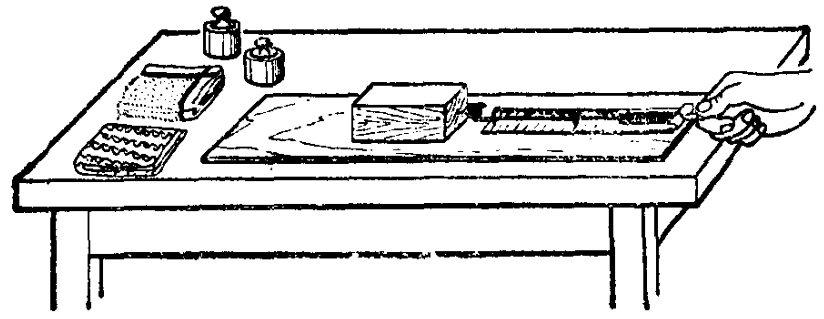
\includegraphics[width=0.5\textwidth]{../pic/czwl1-ch3-12}
    \caption{}\label{fig:3-12}
\end{figure}

(3) 把小木块对长木板的压力和它们之间的摩擦力记入下表。这时木块对木板的压力就等于小木块重。

(4) 在小木块上加一个砝码,用同样的办法测出摩擦力。想想看,这时的压力等于什么。把压力和摩檫力记入下表。

(5) 增加小木块上的砝码,再做一次实验,并且做好记录。

(6) 根据记录的数值,分析一下摩擦力跟压力有什么关系。

\begin{table}[H]
    \centering
    \renewcommand\arraystretch{1.2}
    \begin{tabular}{|w{c}{7em}|*{2}{w{c}{4em}|}}
        \hline
        实验次数 & 压力 & 摩擦力  \\ \hline
        1  & & \\ \hline
        2  & & \\ \hline
        3  & & \\ \hline
    \end{tabular}
\end{table}

(7) 把一块棉布铺在长木板上,小木块上不放砝码,测出这时的摩擦力。

(8) 用毛巾代替棉布,小木块上不放砝码,测出这时的摩擦力。

(9) 比较步驟 (2) 、(7)、(8) 的结果。想想看,在相同的压力下,摩擦力跟什么条件有关系。

